
  \section[Simulations]{GraphSage Simulation Results}
  \label{App:sim_results}

  The results for the GraphSage simulations are presented here. First, the
  results for sum-pooling are presented in figure \ref{fig:sum_sim} and table
  \ref{table:sum_sim}.

  \begin{figure}[htbp!]
		\centering
		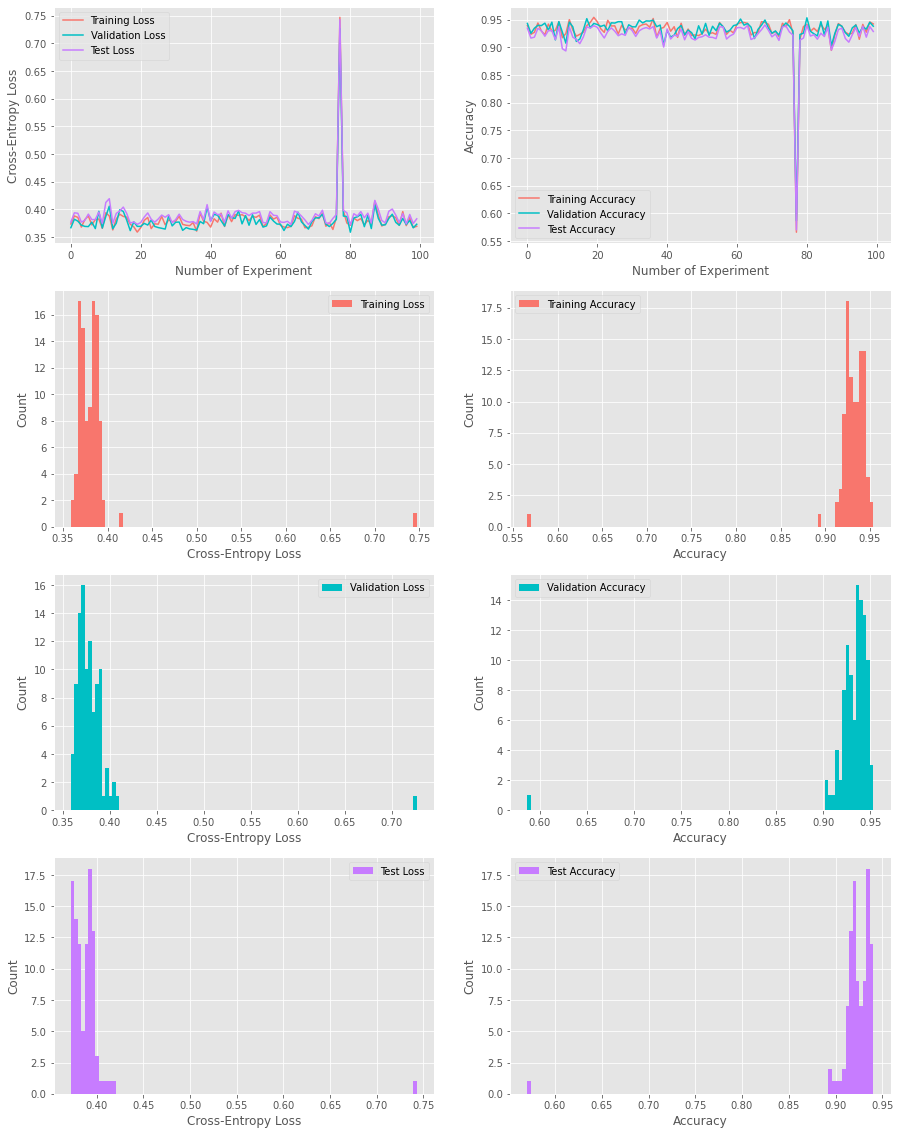
\includegraphics[width=0.9\textwidth]{sum_100_sim.png}
		\caption{Simulations Results Sum-Pooling}
        \label{fig:sum_sim}
  \end{figure}

  \begin{table}[h]
    \centering
      \begin{tabular}{|l||c|c|c|}
      \hline
      \textbf{Metric} & \textbf{Training Set} & \textbf{Validation Set} & 
      \textbf{Test Set}\\
      \hline\hline
      Average Accuracy & 94.63\% & 94.78\% & 93.76\% \\\hline 
                       & (0.46\%) & (0.60\%) & (0.37\%) \\\hline
      Average Cross-Entropy Loss & 0.1346 & 0.1346 & 0.1584 \\\hline
                                 & (0.0109) & (0.0144) & (0.0096) \\
      \hline
    \end{tabular}
    \caption{Simulation Results Sum-Pooling}
    \label{table:sum_sim}
  \end{table}

  \noindent The results for mean aggregation are presented in figure 
  \ref{fig:mean_sim} and table \ref{table:mean_sim}.

  \begin{figure}[h]
		\centering
		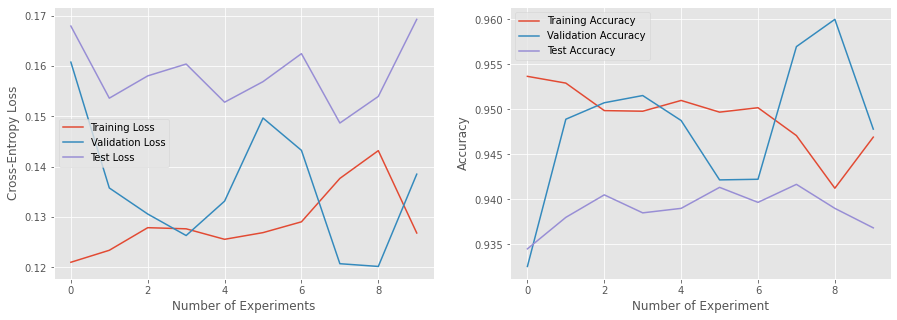
\includegraphics[width=0.9\textwidth]{mean_simulation.png}
		\caption{Simulation Results Mean Aggregation}
        \label{fig:mean_sim}
  \end{figure}

  \begin{table}[h]
    \centering
      \begin{tabular}{|l||c|c|c|}
      \hline
      \textbf{Metric} & \textbf{Training Set} & \textbf{Validation Set} & 
      \textbf{Test Set}\\
      \hline\hline
      Average Accuracy & 94.92\% & 94.82\% & 93.89\% \\\hline 
                       & (0.34\%) & (0.74\%) & (0.20\%) \\\hline
      Average Cross-Entropy Loss & 0.1289 & 0.1359 & 0.1584 \\\hline
                                 & (0.0063) & (0.0121) & (0.0063) \\
      \hline
    \end{tabular}
    \caption{Simulation Results Mean Aggregation}
    \label{table:mean_sim}
  \end{table}

  \noindent The results for LSTM aggregation are lastly presented in figure
  \ref{fig:lstm_sim} and table \ref{table:lstm_sim}. 

  \begin{figure}[h]
		\centering
		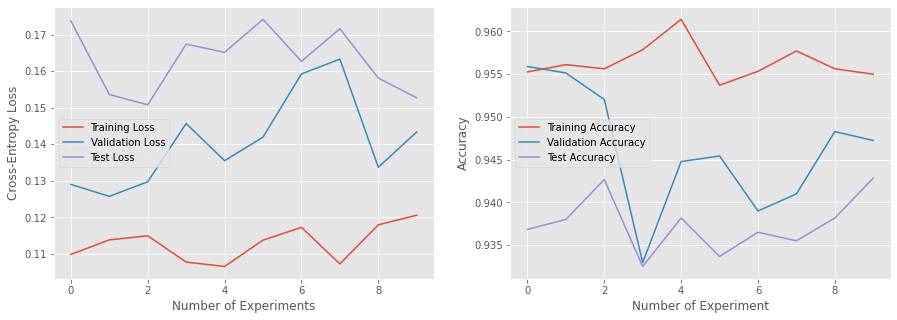
\includegraphics[width=0.9\textwidth]{lstm_sim.png}
		\caption{Simulation Results LSTM Aggregation}
        \label{fig:lstm_sim}
  \end{figure}

  \begin{table}[h]
    \centering
      \begin{tabular}{|l||c|c|c|}
      \hline
      \textbf{Metric} & \textbf{Training Set} & \textbf{Validation Set} & 
      \textbf{Test Set}\\
      \hline\hline
      Average Accuracy & 95.64\% & 94.62\% & 93.75\% \\\hline 
                       & (0.20\%) & (0.69\%) & (0.32\%) \\\hline
      Average Cross-Entropy Loss & 0.1130 & 0.1407 & 0.1630 \\\hline
                                 & (0.0047) & (0.0120) & (0.0084) \\
      \hline
    \end{tabular}
    \caption{Simulation Results LSTM Aggregation}
    \label{table:lstm_sim}
  \end{table}


  \section{Pairplot Feature Data}
  \label{App:pairplot}
  
  The pairplot of the feature data of the US Airline Passenger Data is shown in
  figure \ref{fig:pairplot_feature}.

  \begin{figure}[h]
		\centering
		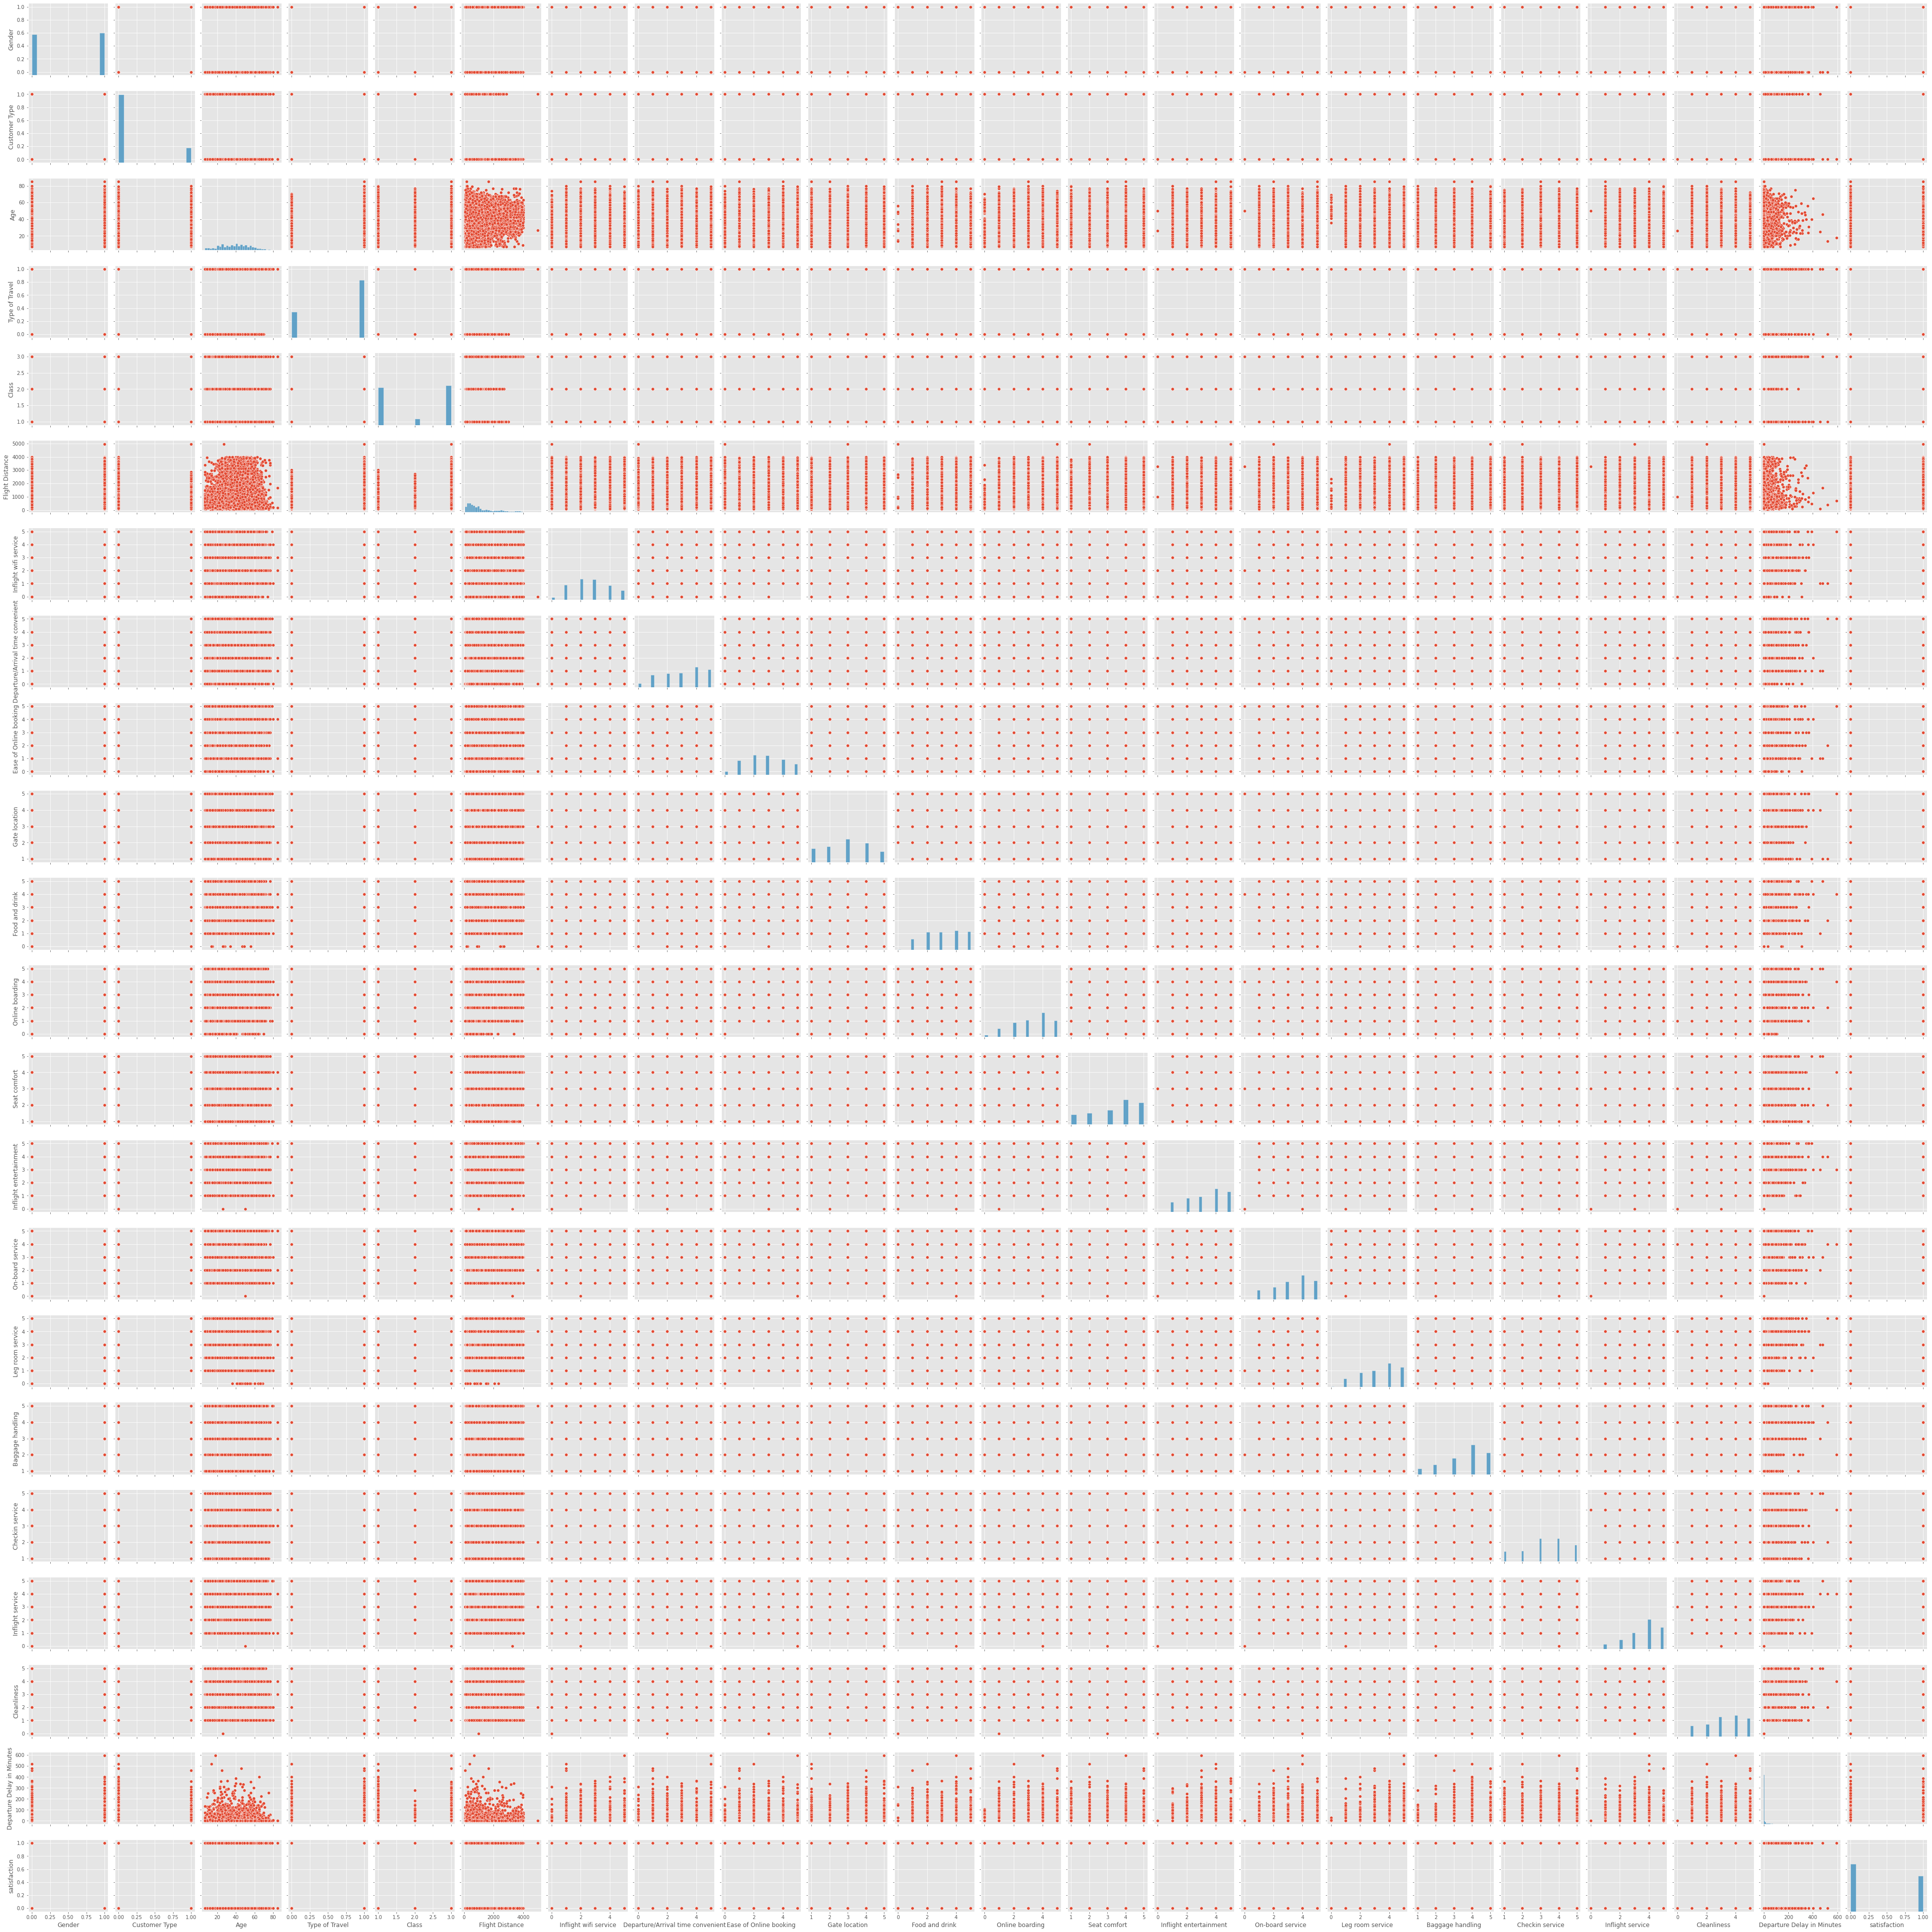
\includegraphics[width=0.9\textwidth]{pariplot_feature_data.png}
		\caption{Pairplot Feature Data US Airline Passenger Data Set}
        \label{fig:pairplot_feature}
  \end{figure}

  \section{ANN Simulation}
  \label{App:ann_sim}

  The results for the ANN were simulated using 10 experiments which trained the
  model for 400 epochs. The results are shown in figure \ref{fig:ann_sim} and 
  table \ref{table:ann_sim}. 

  \begin{figure}[h]
		\centering
		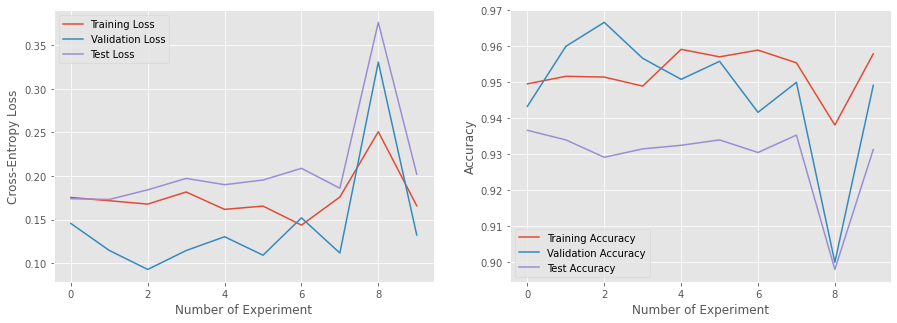
\includegraphics[width=0.9\textwidth]{ANN_sim.png}
		\caption{ANN Simulation Results}
        \label{fig:ann_sim}
  \end{figure}

  \begin{table}[h]
    \centering
      \begin{tabular}{|l||c|c|c|}
      \hline
      \textbf{Metric} & \textbf{Training Set} & \textbf{Validation Set} & 
      \textbf{Test Set}\\
      \hline\hline
      Average Accuracy & 95.28\% & 94.74\% & 92.93\% \\\hline 
                       & (0.61\%) & (1.73\%) & (1.07\%) \\\hline
      Average Cross-Entropy Loss & 0.1760 & 0.1433 & 0.2087 \\\hline
                                 & (0.0268) & (0.0647) & (0.0569) \\
      \hline
    \end{tabular}
    \caption{ANN Simulation Results}
    \label{table:ann_sim}
  \end{table}

